%% This file was edited by Igor Iwakiri
%% Copyright 2019-2020 Elsevier Ltd
%% 
%% This file is part of the 'CAS Bundle'.
%% --------------------------------------
%% 
%% It may be distributed under the conditions of the LaTeX Project Public
%% License, either version 1.2 of this license or (at your option) any
%% later version.  The latest version of this license is in
%%    http://www.latex-project.org/lppl.txt
%% and version 1.2 or later is part of all distributions of LaTeX
%% version 1999/12/01 or later.
%% 
%% The list of all files belonging to the 'CAS Bundle' is
%% given in the file `manifest.txt'.
%% 
%% Template article for cas-dc documentclass for 
%% double column output.



%\documentclass[a4paper,fleqn,longmktitle]{cas-dc}
\documentclass[a4paper,fleqn]{cas-sc}

\usepackage[numbers]{natbib}
%\usepackage[authoryear]{natbib}
\usepackage[authoryear,longnamesfirst]{natbib}
\usepackage[version=4]{mhchem} %So I can write Chemical Reactions like a proper human being
\usepackage{caption}
\usepackage{subcaption}
\usepackage{float}
\usepackage{chngcntr}
\usepackage{xcolor}

%%%Author definitions
%\def\tsc#1{\csdef{#1}{\textsc{\lowercase{#1}}\xspace}}
%\tsc{WGM}
%\tsc{QE}
%\tsc{EP}
%\tsc{PMS}
%\tsc{BEC}
%\tsc{DE}
%%%

% Uncomment and use as if needed
%\newtheorem{theorem}{Theorem}
%\newtheorem{lemma}[theorem]{Lemma}
%\newdefinition{rmk}{Remark}
%\newproof{pf}{Proof}
%\newproof{pot}{Proof of Theorem \ref{thm}}

\begin{document}
\let\WriteBookmarks\relax
\def\floatpagepagefraction{1}
\def\textpagefraction{.001}


%%%%%%%%%%%%%%%%%%%%%%%%%%%%%%%%%%%%%%%%%% Title, and Notes for the whole Paper %%%%%%%%%%%%%%%%%%%%%%%%%%%%%%%%%%%%%%%%%%
% Short title
\shorttitle{Zapdos Database. This Title Will Change.} %CHANGE

% Short author
\shortauthors{I.I. Iwakiri \textit{et al.}} %CHANGE

% Main title of the paper
\title [mode = title]{Zapdos Database. This Title Will Change.} %CHANGE                     

% Title footnote mark
% eg: \tnotemark[1]
%\tnotemark[1,2]

%%%%%%%%%%%%%%%%%%%%%%%%%%%%%%%%%%%%%%%%%% Declaring Authors, Affiliations and Contacts %%%%%%%%%%%%%%%%%%%%%%%%%%%%%%%%%%%%%%%%%%
%%%%%%%%%%%%%%%%%%%%%%%%%%%%%%%%%%%%%%%%%% Authors
% First author
\author[1,2]{Igor Gabriel Ito Iwakiri}[type=editor,
                        orcid=0000-0001-9889-8258]

% Corresponding author indication
\cormark[1]
% Footnote of the first author
%\fnmark[1]

% Email id of the first author
\ead{igor.iwakiri@simoldes.com, igor.g.i.iwakiri@ntnu.no}
% URL of the first author
%\ead[url]{www.website.com}

%  Credit authorship
\credit{Conceptualization, Methodology, Data Analysis, Software, Writing}

%Second Author
\author[1,5]{Luana P. Queiroz}[type=editor,
                        orcid=0000-0003-3092-8136]
% Corresponding author indication
%\cormark[2]
% Footnote of the first author
%\fnmark[2]

% Email id of the first author
\ead{luanaqu@stud.ntnu.no}
% URL of the first author
%\ead[url]{www.website.com}

%  Credit authorship
\credit{Software, Writing}

%%Fourth Author
%\author[3,4]{Lucas J. {dos Santos}}[type=editor,
%                        orcid=0000-0000-0000-0000]
%% Corresponding author indication
%%\cormark[2]
%% Footnote of the first author
%%\fnmark[2]

%% Email id of the first author
%\ead{lucasjs@eq.ufrj.br}
%% URL of the first author
%%\ead[url]{www.website.com}

%%  Credit authorship
%\credit{Software, Review}

\author[3,4]{Amaro G. {Barreto Jr.}}[type=editor,
                        orcid=0000-0000-0000-0000]
% Corresponding author indication
%\cormark[2]
% Footnote of the first author
%\fnmark[2]

% Email id of the first author
\ead{amaro@eq.ufrj.br}
% URL of the first author
%\ead[url]{www.website.com}

%  Credit authorship
\credit{Conceptualization, Review}

%Simoldes Author
\author[2]{Nuno M. Delgado}[type=editor,
                        orcid=0000-0003-0601-8570]
% Corresponding author indication
%\cormark[2]
% Footnote of the first author
%\fnmark[2]

% Email id of the first author
\ead{nuno.delgado@simoldes.com}
% URL of the first author
%\ead[url]{www.website.com}

%  Credit authorship
\credit{Conceptualization, Review}

%Last Author
\author[1]{Idelfonso B. R. Nogueira}[type=editor,
                        orcid=0000-0002-0963-6449]
% Corresponding author indication
%\cormark[2]
% Footnote of the first author
%\fnmark[2]

% Email id of the first author
\ead{idelfonso.b.d.r.nogueira@ntnu.no}
% URL of the first author
%\ead[url]{www.website.com}

%  Credit authorship
\credit{Conceptualization, Review}

%%%%%%%%%%%%%%%%%%%%%%%%%%%%%%%%%%%%%%%%%% Affiliations

% Address/affiliation
\affiliation[1]{organization={Chemical Engineering Department of the Norwegian University of Science and Technology},
    addressline={Gløshaugen}, 
    city={Trondheim},
    % citysep={}, % Uncomment if no comma needed between city and postcode
    %postcode={1043 NX}, 
    % state={},
    country={Norway}}
    
% Address/affiliation
\affiliation[2]{organization={Simoldes Plásticos},
    addressline={R. Comendador António da Silva Rodrigues 165}, 
    city={Oliveira de Azeméis},
    % citysep={}, % Uncomment if no comma needed between city and postcode
    postcode={3720-502}, 
    % state={},
    country={Portugal}}

\affiliation[3]{organization={Escola de Química, EPQB},
    addressline={Universidade Federal do Rio de Janeiro, P.O. Box 68542}, 
    city={Rio de Janeiro, RJ},
    % citysep={}, % Uncomment if no comma needed between city and postcode
    postcode={21941-909}, 
    % state={},
    country={Brazil}}

\affiliation[4]{organization={Programa de Engenharia Química, PEQ/COPPE},
    addressline={Universidade Federal do Rio de Janeiro, PO Box 68502}, 
    city={Rio de Janeiro, RJ},
    % citysep={}, % Uncomment if no comma needed between city and postcode
    postcode={21941-972}, 
    % state={},
    country={Brazil}}

\affiliation[5]{organization={LSRE-LCM, ALiCE},%Department and Organization
            addressline={Faculty of Engineering, University of Porto, Rua Dr. Roberto Frias}, 
            city={Porto},
            postcode={4200-465}, 
            %state={},
            country={Portugal}}

%%%%%%%%%%%%%%%%%%%%%%%%%%%%%%%%%%%%%%%%%% Footnotes
% Title footnote 1.
% eg: \tnotetext[1]{Title footnote text}
% \tnotetext[<tnote number>]{<tnote text>} 
%\tnotetext[1]{This document is the results of the research project funded by the National Science Foundation.}

%\tnotetext[2]{The second title footnote which is a longer text matter to fill through the whole text width and overflow into another line in the footnotes area of the first page.}
   
% For a title note without a number/mark
%\nonumnote{This note has no numbers. In this work we demonstrate $a_b$ the formation Y\_1 of a new type of polariton on the interface between a cuprous oxide slab and a polystyrene micro-sphere placed on the slab.}

% Corresponding author text
\cortext[cor1]{Corresponding author}
%\cortext[cor2]{Principal corresponding author}

% Footnote text
%\fntext[fn1]{This is the first author footnote. but is common to third author as well.}
%\fntext[fn2]{Another author footnote, this is a very long footnote and it should be a really long footnote. But this footnote is not yet sufficiently long enough to make two lines of footnote text.}


%%%%%%%%%%%%%%%%%%%%%%%%%%%%%%%%%%%%%%%%%% Abstract, Keywords, Graphical Abstracts %%%%%%%%%%%%%%%%%%%%%%%%%%%%%%%%%%%%%%%%%%

%%%%%%%%%%%%%%%%%%%%%%%%%%%%%%%%%%%%%%%%%% Highlights %%%%%%%%%%%%%%%%%%%%%%%%%%%%%%%%%%%%%%%%%%
% Research highlights
\begin{highlights}
\item Highlight 1
\item Highlight 2
\item Highlight 3
\end{highlights}

%%%%%%%%%%%%%%%%%%%%%%%%%%%%%%%%%%%%%%%%%% Keywords
% Each keyword is separated by \sep
\begin{keywords}
    Solid-State Electrolytes
    \sep Database
    \sep Conductivity
    \sep Materials Project
\end{keywords}

% Here goes the abstract
\begin{abstract}
    Abstract to be written. We start emphasizing briefly the Databases Available, and their limitations - specially the uniformization i.e. we are never really sure which material we are talking about. Next, we are going to show how more systematic databases such as Materials Project sometimes lack further experimental validation and more "practical" properties such as conductivity. We emphasize the relevance of establishing this link, and the potential of creating Databases that merge the best of both worlds. We end up briefly discussing our toy-project, and the key insights taken out of it.
\end{abstract}

% Use if graphical abstract is present
% \begin{graphicalabstract}
% 
\includegraphics{figs/grabs.pdf}
% \end{graphicalabstract}

%%%%%%%%%%%%%%%%%%%%%%%%%%%%%%%%%%%%%%%%%% Starting the Paper Itself ... %%%%%%%%%%%%%%%%%%%%%%%%%%%%%%%%%%%%%%%%%%%%%%%


\maketitle

\section{Introduction}
Interest in solid-electrolytes (SEs) dates back approximately 200 years to the work of Michael Faraday, with a period of rapid development in the 1960s \cite{zhao2020designing}. In the last decade, SEs have re-emerged as a materials class of notable scientific and commercial interest, standing at the heart of all-solid-state batteries (ASSBs) \cite{famprikis2019fundamentals}. These next-generation electrochemical energy storage systems promise advantages over conventional lithium-ion batteries (LIBs), including enhanced safety due to the non-flammable nature of the SEs, as well as the potential for higher energy and power densities \cite{zhao2020designing, janek2023challenges}. The shift to ASSBs is considered a realistic advancement, with theoretical calculations suggesting a potential specific energy of up to $393 \text{ Wh } \text{kg}^{-1}$ and an energy density of $1,143 \text{ Wh } \text{L}^{-1}$ \cite{janek2023challenges}. However, the core challenge hindering widespread commercial viability is the limited ionic conductivity of many SEs at room temperature (RT), a property that governs charge and discharge rates \cite{zhao2020designing, therrien2025obelix}. While some sulfide-based conductors have achieved ionic conductivities comparable to liquid electrolytes (in the order of $1 \text{ mS } \text{cm}^{-1}$), the discovery of materials with the full suite of required properties, including sufficiently high ionic conductivity, stability against its alkali metal, and suitable mechanical properties, requires a dramatic shift from traditional trial-and-error methods \cite{therrien2025obelix, zhao2020designing, yu2025data}. The high complexity of the materials space makes the exploration and screening of high-performance SEs difficult, as conventional experimental methods and theoretical computations for exhaustive material search are time- and resource-consuming \cite{yang2024dynamic, mishra2023exploring}.


The increasing relevance of SEs in literature is matched by a corresponding demand for robust, machine-readable databases capable of supporting high-throughput and data-driven approaches \cite{yang2024dynamic}. The Materials Genome Initiative (MGI), launched in 2011, endorsed the ambition to computationally predict the existence and basic properties of essentially every single material \cite{armiento2020database}. The resulting trend integrates computational materials science with information technology, spurring the development of resources such as the Materials Project \cite{armiento2020database, jain2013commentary}. Databases are a necessary consequence of modern research, which provides large amounts of digital data that require homogeneous and coherent organization for efficient computer processing and new scientific inferences \cite{grazulis2012crystallography}. Despite this shift, the existing data landscape for solid electrolytes is severely fragmented and inconsistent. Data on critical properties like ionic conductivity are scattered across different scientific papers, and materials frequently lack standardized reporting or unique identifiers. A central challenge in data utilization is the ambiguity concerning the material's identity: "Which material is it?". A single stoichiometric formula can represent multiple distinct crystal structures, each with drastically different electrochemical behavior. Furthermore, literature reports often use different conventions or omit essential metadata. This fragmentation and lack of standardization make it exceedingly difficult to combine data from different sources for comprehensive analysis.


In the materials science domain, the database ecosystem can be broadly divided into generalist and specific platforms. Generalist databases, such as the widely-used, open-access Materials Project (MP), the Crystallography Open Database (COD), and the proprietary Inorganic Crystal Structure Database (ICSD), offer vast collections of structural and computed material properties \cite{armiento2020database}. The Materials Project, for instance, provides an open dataset generated via high-throughput computing to uncover the properties of inorganic materials \cite{jain2013commentary}, currently holding computed data for more than 70,000 materials and millions of associated properties \cite{ye2018harnessing}, and offering a high-level of uniformity and versatility. However, these generalist platforms often do not prioritize, or systematically include, the key experimentally verified solid-state electrolyte properties, such as ionic conductivity, that are crucial for materials screening. Conversely, specific SSE databases, like the Dynamic Database of Solid-State Electrolytes (DDSE) \cite{yang2024dynamic}, the Liverpool Ionics (LiIon) Dataset \cite{hargreaves2023database}, the OBELiX dataset \cite{therrien2025obelix}, and the dataset from Shon et al. (2023) \cite{shon2023extracting}, focus on gathering these relevant experimental properties. While invaluable, these databases are typically smaller, lack uniformity, and do not provide the wealth of pre-calculated theoretical and structural descriptors found in generalist platforms. For instance, many experimental SSE databases contain limited structural information: the DDSE and Shon and Min databases contain only a qualitative structure description for some materials, the LiIon dataset only includes the structural family, and the Laskowski dataset is limited to space group information, making it difficult to train ML models that require a full crystal description \cite{therrien2025obelix}. A high-level comparison of these database types is provided in Table \ref{tab:database_comparison} below.

\begin{table}[h]
    \centering
    \caption{Comparative Overview of Select Material Databases}
    \label{tab:database_comparison}
    \renewcommand{\arraystretch}{1.3}
    \begin{tabular}{p{1.9cm}p{2.8cm}p{2cm}p{2.5cm}p{3.6cm}}
        \toprule
        \textbf{Database} & \textbf{Primary Content Focus} & \textbf{Access} & \textbf{Source of Data} & \textbf{Key Distinguishing Feature} \\
        \midrule
        Materials Project (MP) \cite{ye2018harnessing,armiento2020database} & Inorganic Crystalline Solids and Molecular Species \cite{ spotte2023database} & Open & High-Throughput DFT, Computational & Massive scale and consistent theoretical properties \\
        ICSD \cite{hellenbrandt2004inorganic, zagorac2019recent} & Inorganic Crystal Structures (since 1913)  & Restricted and Commercial & Experimental & Exhaustive collection of experimental inorganic structures \\
        Crystallography Open Database (COD) \cite{grazulis2012crystallography} & Small/Medium Unit Cell Crystal Structures & Open & Experimental & Open-access, collaborative repository of 'small molecule' structures \\
        DDSE \cite{yang2024dynamic, yang2024user} & Inorganic and Polymer SSEs (various cations)  & Restricted  & Experimental and Computational  & Dynamic data mining from experimental reports\\
        OBELiX \cite{therrien2025obelix} & Lithium Solid-State Electrolytes  & Open  & Expert-Curated Experimental ACIS  & Curated experimental $\sigma_{RT}$ and full crystal structure descriptions (CIFs) \\
        LiIon Dataset \cite{hargreaves2023database, durdy2023liverpool}  & Lithium-ion Conductors  & Open & Expert-Curated Experimental ACIS  & Focus on Li-ion conductivity measured by a.c. impedance spectroscopy\\
        \bottomrule
    \end{tabular}
\end{table}

The next frontier of materials discovery is harnessing computational information for automated learning and accelerated discovery \cite{ye2018harnessing}. Machine learning (ML) has emerged as an effective and trustworthy tool for screening new functional materials and predicting desirable properties like ionic conductivity \cite{yang2024dynamic, yu2025data, mishra2023exploring}. The accuracy of an ML model, however, depends critically on the quality and quantity of the training data \cite{hargreaves2023database}. The current fragmented state of SSE data is a major hindrance to developing reliable ML models. First, mislabeled or ambiguous data, where a composition corresponds to different phases or doped variants, is a critical barrier for ML applications, where errors can easily propagate across predictive models. Second, ML models require comprehensive input features that describe not only the composition but also the underlying crystal structure (e.g., lattice parameters, space group, and even atomic positions or partial occupancy) \cite{therrien2025obelix, mishra2023exploring}. While composition-only models are important for screening unexplored chemical space, models built with full structure and composition are generally superior in performance \cite{hargreaves2023database}. The lack of precise structural information labeled with experimental ionic conductivity makes it difficult both to compare experimental values with theoretical predictions and to train high-accuracy ML models \cite{therrien2025obelix}. Third, the manual and expert-driven process required to collect and curate high-quality experimental data is complex and time-consuming, resulting in datasets that are typically very small for ML standards (often fewer than 10,000 entries) \cite{hargreaves2023database}. This low-data regime highlights the necessity for new, densely-featured datasets to inform more sophisticated ML frameworks \cite{therrien2025obelix}.


In this work, the developers address this fundamental challenge by harmonizing three open-access datasets of experimentally reported solid-state electrolytes (OBELiX, LiIon, and the Shon et al. (2023) \cite{shon2023extracting}) against the rigorously defined entries of the Materials Project. This process establishes the crucial, unambiguous link between experimental performance data and high-quality, standardized structural and theoretical descriptors. The work's approach involved picking up three of the most relevant Specific Databases and using the properties available in each one to link them to specific entries (IDs) of Material Project. The rationale was not only to know which exact material the specific databases were addressing but also to bridge it with so many relevant, theoretical (calculated through MD or DFT) properties from Materials Project. A scoring system was applied to quantify the reliability of the formula-to-structure matches. By providing a versatile, uniform, and experimentally verified database, this work is expected to unlock several possibilities of work that were restricted due to the lack of relevant SSE properties in the Generalist Databases or lack of standardization in the Specific Databases. The unified framework enables researchers to dynamically select high-confidence or broad datasets, tailored to different ML tasks such as training, validation, or benchmarking.



\section{Data Process and Cleaning}


The technical construction of the harmonized solid-state electrolyte (SSE) database began with a bottom-up approach, necessitating the meticulous cleaning and standardization of data derived exclusively from open-access source databases. These sources included Materials Project (MP) \cite{jain2013commentary}, OBELiX \cite{therrien2025obelix}, the Liverpool Ionics Dataset \cite{durdy2023liverpool, hargreaves2023database}  and the specialized dataset from Shon et al. (2023) \cite{shon2023extracting}. This process involved the critical first step of mapping all raw entries to a uniform data structure defined by seven key properties. For each entry, the "Specific ID" was extracted to maintain traceability to the source database, alongside the experimentally measured "Conductivity" value and the corresponding "DOI" of the original publication. Structural details were recorded via the reported "Space Group" and any provided ".CIF File" (or sufficient information to generate it), which represents the material's geometry. Finally, the "Temperature" at which the measurement occurred and any existing "Generalist ID" (where a source database already established a direct link to a general database ID) were collected. If a specific property was not provided by the source database, the corresponding field was initially left blank.


The subsequent phase addressed the standardization of structural information, a necessity given the frequent absence of a definitive space group in the experimental databases, which would otherwise drastically reduce the capacity for unique material identification. To circumvent this, the methodology leveraged supplementary information, specifically the material's Family Cluster (e.g., Garnet, Perovskite, or NASICON type) when available. By relying on established crystallographic knowledge for each structural family, it was possible to infer the most probable space group (SG) or a manageable subgroup of possibilities. For instance, materials identified as belonging to the high-symmetry Garnet family were primarily assumed to possess the space group $Ia\bar{3}d (230)$, while the NASICON family allowed for a defined range of SGs, including $R\bar{3}c (167)$, $R\bar{3} (148)$, or $C2/c (15)$, which served as crucial filtering criteria in the subsequent matching phase. This structural inference was only applied to presumed crystalline materials; entries categorized as "Glass" or "Glass-Ceramic," which are amorphous, were noted as not having a presence in the crystalline-focused Materials Project and were consequently excluded from the MP matching phase. The full set of assumptions regarding family clusters and their likely space groups is summarized in Table \ref{tab:family_clusters_sg}.

\begin{table}[htbp]
    \centering
    \caption{Overview of family clusters and their likely space groups (SG).}
    \label{tab:family_clusters_sg}
    \begin{tabular}{ll}
        \hline
        \textbf{Family Cluster} & \textbf{Likely SG} \\
        \hline
        Rocksalt          & Fm$\bar{3}$m (225) \\
        Anti-Perovskite   & Pm$\bar{3}$m (221); Pnma (62); P1 (1) \\
        Argyrodite        & F$\bar{4}$3m (216); Pna21 (33); \\
        LISICON           & Pmn21 (31); P1 (1); R$\bar{3}$ (148); \\
        Zircon            & I41/amd (141) \\
        Garnet            & Ia$\bar{3}$d (230) \\
        Thio-LISICON      & Pnma (62); Pmn21 (31); P21/m (11) \\
        Perovskite        & Pm$\bar{3}$m (221); Pnma (62); Amm2 (38) \\
        NASICON           & R$\bar{3}$c (167); R$\bar{3}$ (148); C2/c (15); P21/c (14); P1 (1) \\
        Glass             & Amorphous i.e. Not present in Materials Project\\
        Lysonite          & Not well established - Left Blank \\
        Olivine           & Pbnm (62) \\
        Phenakite         & R$\bar{3}$ (148) \\
        Glass-Ceramic     & Amorphous* i.e. Not present in Materials Project\\
        Other             & Not well established - Left Blank\\
        \hline
    \end{tabular}
\end{table}


The second core stage of cleaning addressed internal inconsistencies and format errors within the raw data columns, with primary focus on the chemical formula and the conductivity values. To ensure that the composition was deterministically identifiable regardless of the source database’s input ordering (e.g., $Li_{6}La_{2}CaNb_{2}O_{12}$ versus $Li_{6}CaLa_{2}Nb_{2}O_{12}$), the Python Materials Genomics (pymatgen) library \cite{ong2013python} was integrated into the pipeline. Specifically, the pipeline invoked the normalize\_formula function to instantiate a pymatgen.core.Composition object and emit its reduced\_formula, guaranteeing a deterministic, alphabetized stoichiometry (e.g., $CaLa_{2}Li_{6}Nb_{2}O_{12}$). Entries that lacked a proper chemical formula, such as those only named "Polyethylene oxide" or generalized names like "NASICON," were classified as Underdefined Formulae and not considered. This exclusion was critical because while a "classic" formula exists for NASICON ($\text{Na}_{1+x}\text{Zr}_2\text{Si}_x\text{P}_{3-x}\text{O}_{12}$), the term often refers to numerous doped variants in literature, and without further verification, automated matching is unreliable.


Finally, the integrity of the crucial Conductivity value required extensive normalization due to highly inconsistent reporting styles. Several string-based values and notational errors had to be programmatically converted to a unified numerical form. Simple errors, such as a leading dash in cases like $-10^{-10}$, were resolved by removing the dash and interpreting the value as $10^{-10}$. Entries reported as strings (e.g., "$1.0 \times 10^{-7}$") were converted to a float type. More intricate processing was required for values representing ranges or averages: when an entry provided multiple conductivity values as a series or range (e.g., "2.6 $\times 10^{-3}$ and 1.4 $\times 10^{-3}$" or "0.154 to 0.045"), the logarithmic average of the endpoints was computed to generate a single representative value. In cases where only a maximum bound was given (e.g., "to $1.8 \times 10^{-4}$"), that value was adopted directly. Furthermore, noisy or garbled entries, such as "$10^{-5}-1 \times 10^{-6}$" (which required manual DOI checking to confirm the authors intended "$10^{-5} \sim 10^{-6}$"), were resolved by calculating the logarithmic average. This meticulous, multi-stage cleaning and normalization process, schematically summarized in Figure \ref{fig:datacleaning}, was essential to ensure that every remaining entry possessed a verifiable composition and a singular, standardized numerical value for ionic conductivity, making the data fit for high-throughput matching and predictive modeling.

\begin{figure*}
    \centering
    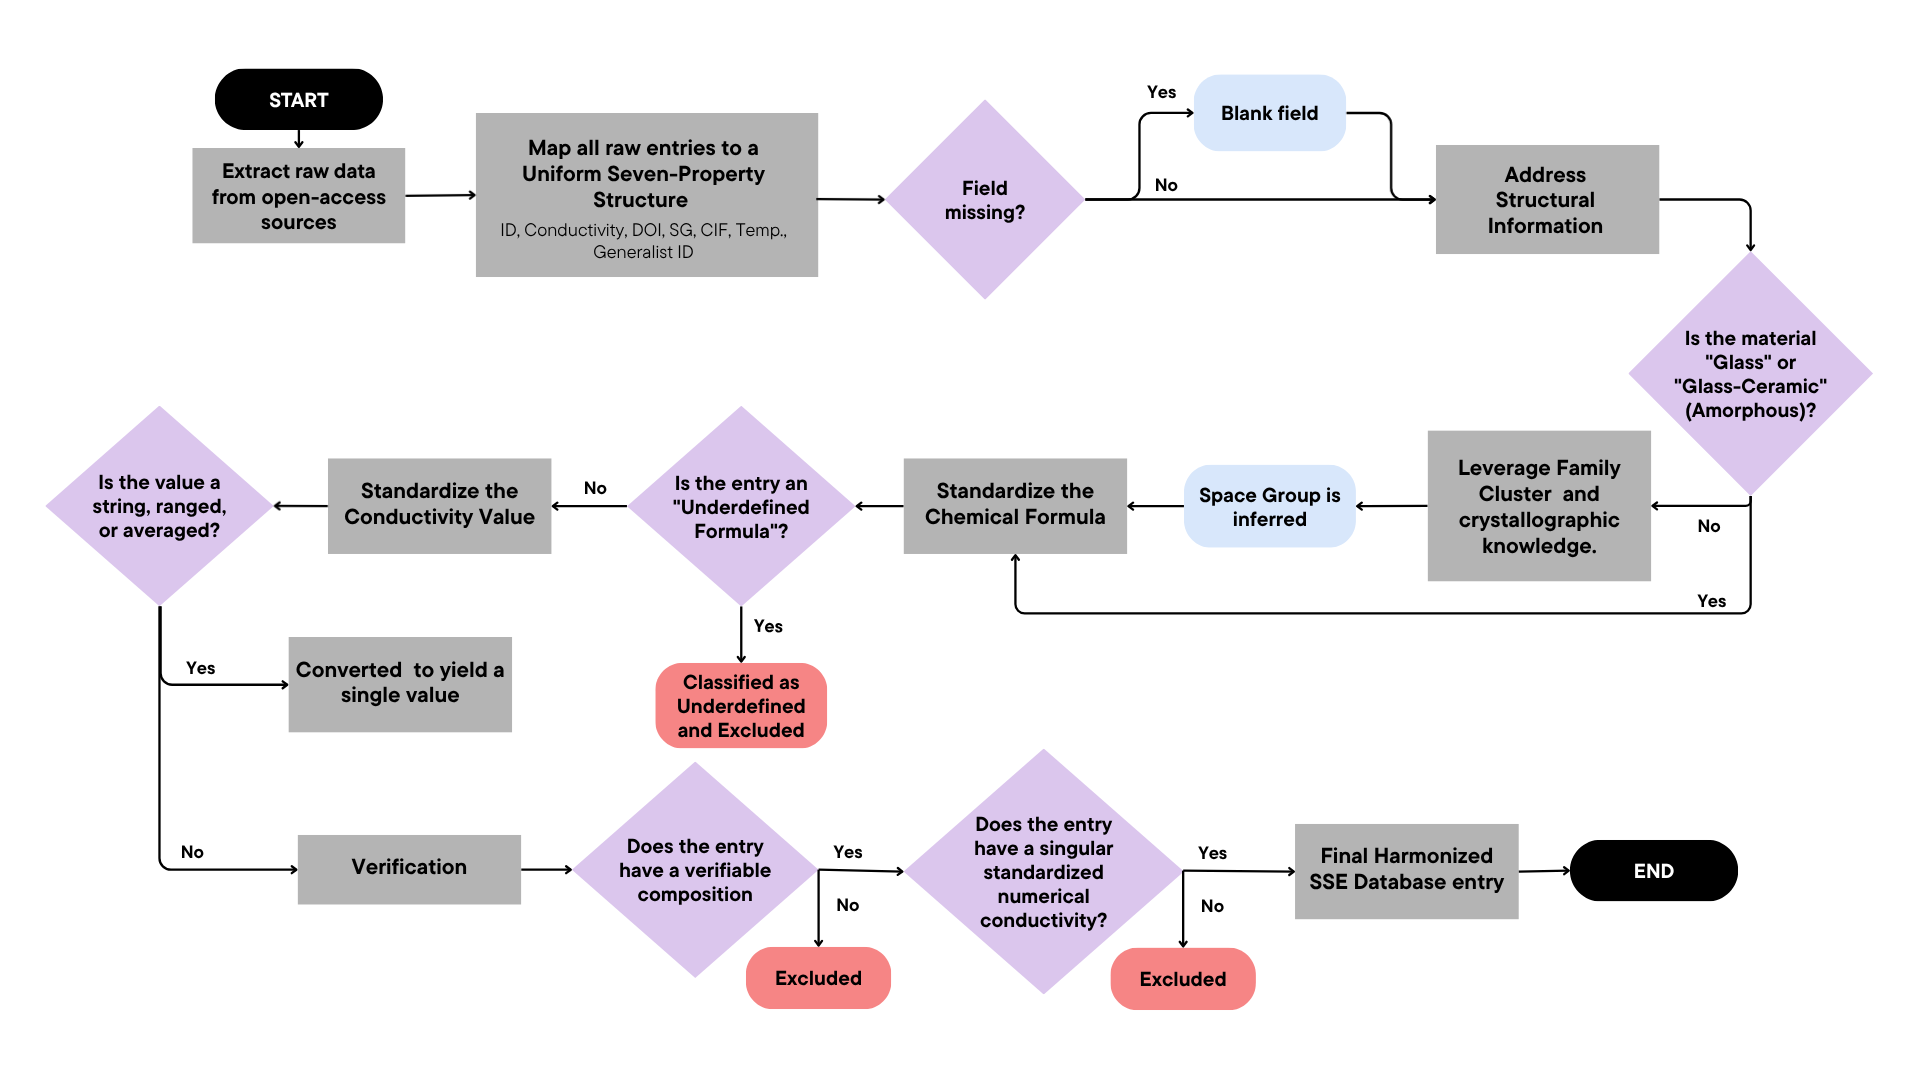
\includegraphics[width=1\linewidth]{figs/datacleaning.png}
    \caption{Flowchart of the technical cleaning and standardization process for the Solid-State Electrolyte (SSE) database.}
    \label{fig:datacleaning}
\end{figure*}

\section{Matching Methodology and Tiers}

A hierarchical, multi-stage matching algorithm was developed to cross-reference entries from the Specific Databases with the Materials Project database. This process assigns a tiered evidence model, combining database identifiers, crystal symmetry, and structural isomorphism.

The primary matching criterion employed the presence of a Generalistic ID, such as the Inorganic Crystal Structure Database (ICSD) accession number as a direct provenance link. For each entry, the corresponding identifier was queried against the Materials Project database using the MaterialsProjectAPI.by\textunderscore icsd routine. This function interrogates the MP summary documentation and compares the database\textunderscore IDs.icsd field of each returned document against the source identifier.
An exact numerical match was considered a definitive link between the datasets. 

For entries lacking a successful match, a secondary step was implemented where candidate MP structures were retrieved via MaterialsProjectAPI.structures\textunderscore for and compared directly against the entry's CIF file. Both structures were parsed into pymatgen.Structure objects and evaluated using the StructureMatcher algorithm, also part of the pymatgen library.
A tiered tolerance-based approach was implemented to assess isomorphism. The StructureMatcher was applied (site tolerance ltol = 0.2, stoichiometric tolerance stol = 0.3, and angle\textunderscore tol = 5°). This stage provided auditable crystallographic equivalence independent of symmetry labeling, with the specific CIF path recorded as provenance.
This hierarchical methodology thus integrates explicit database identifiers, symmetry-aware compositional filters, and geometry-based confirmation to ensure each entry is matched to Materials Project records with explainable evidence.

Finally, as a tertiary step, the chemical composition of each entry was canonicalized to its reduced formula using the pymatgen.Composition().reduced\textunderscore formula method from the pymatgen library. This reduced formula was subsequently used to query the MP database via the MaterialsProjectAPI.by\textunderscore formula function, retrieving all MP summary documents sharing the identical reduced formula. 
For this new pool of candidates, space-group symbols from both the MP candidate and the entry of the Specific Database were normalized (\textit{e.g.}, whitespace removal, hyphen standardization). This way, it was possible to find candidates with not only share an exact identical reduced formula, but also an exact match in its normalized space-group symbol or number.
If no exact space-group match was found, a broader comparison at the crystal system level was performed. The lattice system (\textit{e.g.}, triclinic, monoclinic, orthorhombic) for the entry was inferred from its space-group number using a standard lookup function (crystal\textunderscore system\textunderscore from\textunderscore number), therefore allowing effectively grouping materials within the same crystal family (\textit{e.g.}, P1 and P-1) that may have different space-group assignments.

Finally, after the comparison, every entry that was matched with an mp-id were classified in different tiers based on how rigorous this match occurred. For instance:

\textbf{Tier 0:} Destined to entries that presented a Generalistic ID that could directly lead to an mp-id, or else, that presented a DOI that were related to a specific mp-id. 

\textbf{Tier 1:} Destined to entries that were matched through the .CIF comparison \textit{i.e.} the geometry presented in the Specific Database were correspondent to the geometry presented in the Materials Project Database.

\textbf{Tier 2:} Destined to entries that were matched through not only an exact chemical formula, but also is registered in the Materials Project with the same Space Group according to Table \ref{tab:family_clusters_sg}.

\textbf{Tier 3:} Destined to entries with an exact chemical formula and, even though the space group was different to the one registered in the Materials Project, both of them would share the same lattice system \textit{e.g.} monoclinic.

\textbf{Tier 4:} Destined to entries with an exact chemical formula, but the space group is not even in the same lattice system as the entry in Materials Project.

\begin{itemize}
    \item Luana's version
\end{itemize}

The unification of the cleaned experimental dataset with the Materials Project (MP) records was executed through a hierarchical, multi-stage matching algorithm, outlined in Figure \ref{fig:hierarch}, which systematically cross-referenced entries from the specific open-access sources with the comprehensive MP database. This process was designed to assign a tiered evidence model, combining database identifiers, crystal symmetry, and structural isomorphism.

\begin{figure*}
    \centering
    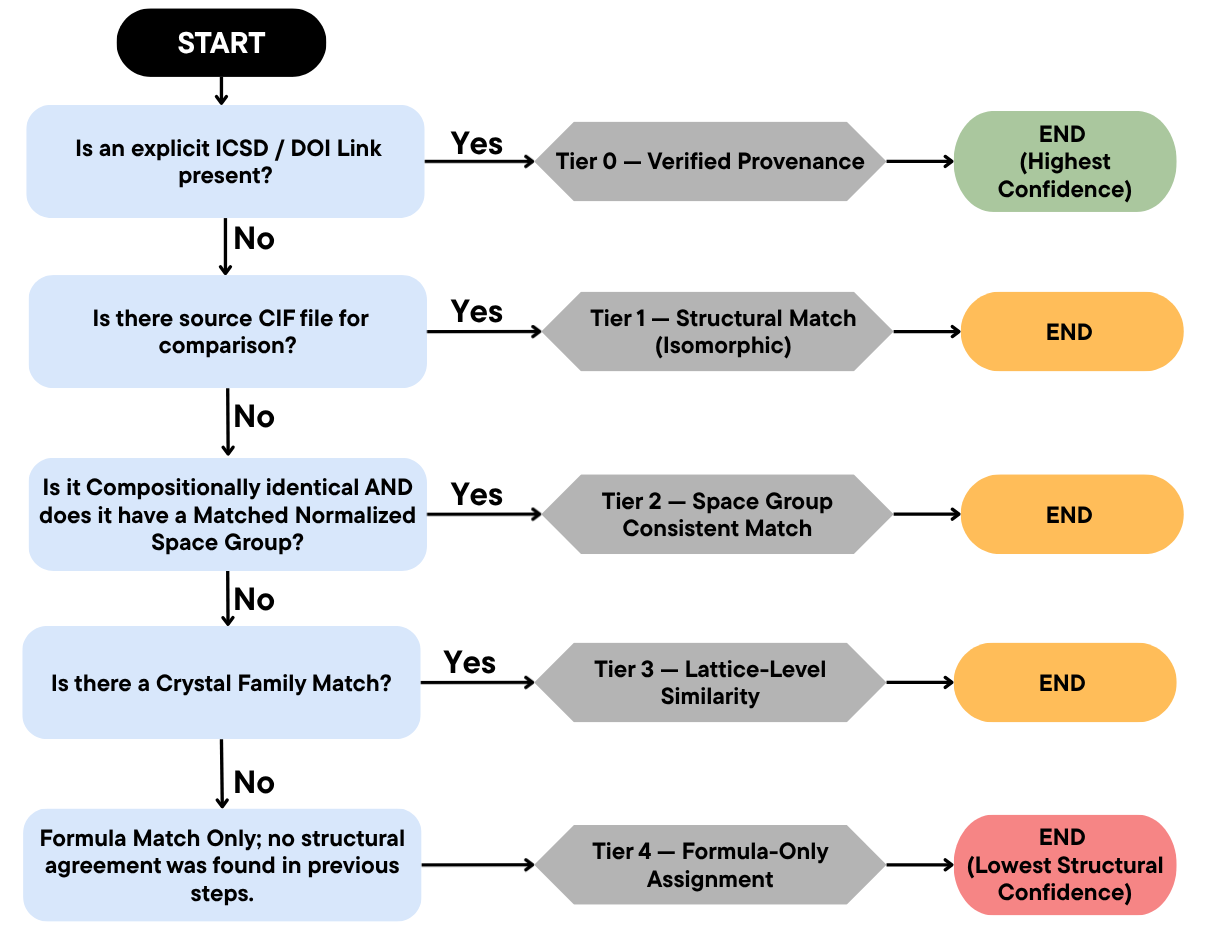
\includegraphics[width=0.7\linewidth]{figs/hierarch.png}
    \caption{Hierarchical Matching Methodology and Confidence Tier Assignment.}
    \label{fig:hierarch}
\end{figure*}

The algorithm's execution begins with the Direct Identifier Provenance (Tier 0). This primary matching criterion employs the presence of a Generalistic ID, such as the Inorganic Crystal Structure Database (ICSD) accession number, as a direct provenance link. For each entry, the corresponding identifier is programmatically queried against the Materials Project using the specific routine, MaterialsProjectAPI.by\_icsd. This function interrogates the MP summary documentation and compares the database\_IDs.icsd field of each returned document against the source identifier. An exact numerical match is considered a definitive link between the datasets. Tier 0 is consequently destined for entries that presented a Generalistic ID that could directly lead to an MP-ID, or else, that presented a DOI that was related to a specific MP-ID.

For entries failing the provenance check, the second stage implements a Geometric Isomorphism Test (Tier 1). This requires the availability of the entry's Crystal Information File (CIF). Candidate MP structures are retrieved via the MaterialsProjectAPI.structures\_for command and compared directly against the experimental entry's CIF file. Both structures are parsed into pymatgen.Structure objects and rigorously evaluated using the StructureMatcher algorithm, also part of the Pymatgen library. A tiered tolerance-based approach is utilized to assess isomorphism: the StructureMatcher is applied with a site tolerance ($ltol$) of $0.2$, a stoichiometric tolerance ($stol$) of $0.3$, and an angle tolerance ($angle\_tol$) of $5^{\circ}$. This stage provides auditable crystallographic equivalence independent of symmetry labeling, with the specific CIF path recorded as provenance. Tier 1 is destined for entries that were matched through this CIF comparison, meaning the geometry presented in the specific database was correspondent to the geometry presented in the Materials Project Database.

The final and broadest stage involves Symmetry-Aware Formula Matching (Tiers 2, 3, 4). This stage begins by canonicalizing the chemical composition of each entry to its reduced formula using the pymatgen.Composition().reduced\_formula method. This formula is used to query all MP records via the MaterialsProjectAPI.by\_formula function, creating a pool of compositionally identical candidates. This pool is filtered using two sequential symmetry criteria:

\begin{enumerate}
    \item Exact Space Group Match (Tier 2): Space-group symbols from both the MP candidate and the experimental entry (including the inferred SGs from Table 2) are normalized via whitespace removal and hyphen standardization. An exact match between the normalized symbols signifies high probability of structural correspondence, assigning the entry to Tier 2.
    \item Lattice System Match (Tier 3): If no exact space-group match was found, a broader comparison at the crystal system level was performed. The lattice system (e.g., triclinic, monoclinic, orthorhombic) for the entry was inferred from its space-group number using a standard lookup function (crystal\_system\_from\_number). This allows effectively grouping materials within the same crystal family (e.g., $P1$ and $P\bar{1}$) that may have different space-group assignments. If the MP candidate shares this same lattice system, the entry is assigned Tier 3. Tier 3 is destined for entries with an exact chemical formula where, even though the space group was different, both the experimental entry and the MP record share the same lattice system (e.g., monoclinic).
\end{enumerate}


The remaining entries, which possess an exact chemical formula but whose space group is not even in the same lattice system as the entry in Materials Project, are classified into the lowest confidence level. Tier 4 is destined for these entries. This hierarchical methodology thus integrates explicit database identifiers, symmetry-aware compositional filters, and geometry-based confirmation to ensure each entry is matched to Materials Project records with explainable evidence.

\section{Dataset Overview and Statistics}
The idea here is Igor presenting several graphs to facilitate a reader to understand exactly how our Ultimate Database ended up being.
Some ideas:
\begin{itemize}
    \item \textbf{Tier Distribution:} Pie Chart showing fraction of entries in each Tier; Stacked bar showing which Specific DB contributes more for each tier.
    \item \textbf{Property Coverage:} Histogram of Temperatures Covered; Conductivity Distribution for Each Family Cluster; 
    \item \textbf{Cluster Frequency:} Pie chart per families; Pie chart per Lattice Systems; Heatmap of Element Occurrence; 
\end{itemize}

\section{Case Study}
To demonstrate practical accessibility of the unified database, we deployed a local Retrieval-Augmented Generation (RAG) service that allows natural-language queries against the CSV dataset. This section illustrates representative examples and evaluates whether retrieved answers preserve factual provenance.

\subsection{Methodology}
Hello World.
\subsection{Results and Discussion}
Hello World.

\section{Conclusion}
Hello World.

\section{Tasks da Luana - Isso Será Apagado Depois}
\begin{itemize}
    \item Figure for "Data Processing and Cleaning". \textbf{(Done)}
    \item Figure for "Matching Methodology and Tiers". \textbf{(Done)}
    \item Figure for RAG pipeline diagram (Database → Embedding → FAISS → LLM → Answer with IDs).
    \item Help me to transform the "informal" texts into the actual stuff. All the info is already there. Start with Introduction. Then, go to Data Cleaning. 
    

\end{itemize}

%\appendix
%\section{My Appendix}
%Appendix sections are coded under \verb+\appendix+.

%\verb+\printcredits+ command is used after appendix sections to list 
%author credit taxonomy contribution roles tagged using \verb+\credit+ 
%in frontmatter.

\printcredits

\section*{Acknowledgements}
This work was financially supported by Fundação para a Ciência e a Tecnologia, I.P. /MCTES through national funds: UI/BD/154743/2023 (DOI: 10.54499/UI/BD/154743/2023), LSRE-LCM, UID/50020/2025; and ALiCE, LA/P/0045/2020 (DOI: 10.54499/LA/P/0045/2020).

%% Loading bibliography style file
%\bibliographystyle{model1-num-names}
\bibliographystyle{cas-model2-names}

% Loading bibliography database
\bibliography{cas-refs.bib}


\end{document}




These are some instructions left from the Elsevier Template.
\section{Introduction}

The Elsevier cas-dc class is based on the
standard article class and supports almost all of the functionality of
that class. In addition, it features commands and options to format the
\begin{itemize} \item document style \item baselineskip \item front
matter \item keywords and MSC codes \item theorems, definitions and
proofs \item lables of enumerations \item citation style and labeling.
\end{itemize}

This class depends on the following packages
for its proper functioning:

\begin{enumerate}
\itemsep=0pt
\item {natbib.sty} for citation processing;
\item {geometry.sty} for margin settings;
\item {fleqn.clo} for left aligned equations;
\item {graphicx.sty} for graphics inclusion;
\item {hyperref.sty} optional packages if hyperlinking is
  required in the document;
\end{enumerate}  

All the above packages are part of any
standard \LaTeX{} installation.
Therefore, the users need not be
bothered about downloading any extra packages.

\section{Installation}

The package is available at author resources page at Elsevier
(\url{http://www.elsevier.com/locate/latex}).
The class may be moved or copied to a place, usually,\linebreak
\verb+$TEXMF/tex/latex/elsevier/+, %$%%%%%%%%%%%%%%%%%%%%%%%%%%%%
or a folder which will be read                   
by \LaTeX{} during document compilation.  The \TeX{} file
database needs updation after moving/copying class file.  Usually,
we use commands like \verb+mktexlsr+ or \verb+texhash+ depending
upon the distribution and operating system.

\section{Front matter}

The author names and affiliations could be formatted in two ways:
\begin{enumerate}[(1)]
\item Group the authors per affiliation.
\item Use footnotes to indicate the affiliations.
\end{enumerate}
See the front matter of this document for examples. 
You are recommended to conform your choice to the journal you 
are submitting to.

\section{Bibliography styles}

There are various bibliography styles available. You can select the
style of your choice in the preamble of this document. These styles are
Elsevier styles based on standard styles like Harvard and Vancouver.
Please use Bib\TeX\ to generate your bibliography and include DOIs
whenever available.

Here are two sample references: 
\cite{Fortunato2010}
\cite{Fortunato2010,NewmanGirvan2004}
\cite{Fortunato2010,Vehlowetal2013}

\section{Floats}
{Figures} may be included using the command,\linebreak 
\verb+\includegraphics+ in
combination with or without its several options to further control
graphic. \verb+\includegraphics+ is provided by {graphic[s,x].sty}
which is part of any standard \LaTeX{} distribution.
{graphicx.sty} is loaded by default. \LaTeX{} accepts figures in
the postscript format while pdf\LaTeX{} accepts {*.pdf},
{*.mps} (metapost), {*.jpg} and {*.png} formats. 
pdf\LaTeX{} does not accept graphic files in the postscript format. 

\begin{figure}
	\centering
		
\includegraphics[scale=.75]{figs/Fig1.pdf}
	\caption{The evanescent light - $1S$ quadrupole coupling
	($g_{1,l}$) scaled to the bulk exciton-photon coupling
	($g_{1,2}$). The size parameter $kr_{0}$ is denoted as $x$ and
	the \PMS is placed directly on the cuprous oxide sample ($\delta
	r=0$, See also Table \protect\ref{tbl1}).}
	\label{FIG:1}
\end{figure}


The \verb+table+ environment is handy for marking up tabular
material. If users want to use {multirow.sty},
{array.sty}, etc., to fine control/enhance the tables, they
are welcome to load any package of their choice and
{cas-dc.cls} will work in combination with all loaded
packages.

\begin{table}[width=.9\linewidth,cols=4,pos=h]
\caption{This is a test caption. This is a test caption. This is a test
caption. This is a test caption.}\label{tbl1}
\begin{tabular*}{\tblwidth}{@{} LLLL@{} }
\toprule
Col 1 & Col 2 & Col 3 & Col4\\
\midrule
12345 & 12345 & 123 & 12345 \\
12345 & 12345 & 123 & 12345 \\
12345 & 12345 & 123 & 12345 \\
12345 & 12345 & 123 & 12345 \\
12345 & 12345 & 123 & 12345 \\
\bottomrule
\end{tabular*}
\end{table}

\section[Theorem and ...]{Theorem and theorem like environments}

{cas-dc.cls} provides a few shortcuts to format theorems and
theorem-like environments with ease. In all commands the options that
are used with the \verb+\newtheorem+ command will work exactly in the same
manner. {cas-dc.cls} provides three commands to format theorem or
theorem-like environments: 

\begin{verbatim}
 \newtheorem{theorem}{Theorem}
 \newtheorem{lemma}[theorem]{Lemma}
 \newdefinition{rmk}{Remark}
 \newproof{pf}{Proof}
 \newproof{pot}{Proof of Theorem \ref{thm2}}
\end{verbatim}


The \verb+\newtheorem+ command formats a
theorem in \LaTeX's default style with italicized font, bold font
for theorem heading and theorem number at the right hand side of the
theorem heading.  It also optionally accepts an argument which
will be printed as an extra heading in parentheses. 

\begin{verbatim}
  \begin{theorem} 
   For system (8), consensus can be achieved with 
   $\|T_{\omega z}$ ...
     \begin{eqnarray}\label{10}
     ....
     \end{eqnarray}
  \end{theorem}
\end{verbatim}  


\newtheorem{theorem}{Theorem}

\begin{theorem}
For system (8), consensus can be achieved with 
$\|T_{\omega z}$ ...
\begin{eqnarray}\label{10}
....
\end{eqnarray}
\end{theorem}

The \verb+\newdefinition+ command is the same in
all respects as its \verb+\newtheorem+ counterpart except that
the font shape is roman instead of italic.  Both
\verb+\newdefinition+ and \verb+\newtheorem+ commands
automatically define counters for the environments defined.

The \verb+\newproof+ command defines proof environments with
upright font shape.  No counters are defined. 


\section[Enumerated ...]{Enumerated and Itemized Lists}
{cas-dc.cls} provides an extended list processing macros
which makes the usage a bit more user friendly than the default
\LaTeX{} list macros.   With an optional argument to the
\verb+\begin{enumerate}+ command, you can change the list counter
type and its attributes.

\begin{verbatim}
 \begin{enumerate}[1.]
 \item The enumerate environment starts with an optional
   argument `1.', so that the item counter will be suffixed
   by a period.
 \item You can use `a)' for alphabetical counter and '(i)' 
  for roman counter.
  \begin{enumerate}[a)]
    \item Another level of list with alphabetical counter.
    \item One more item before we start another.
    \item One more item before we start another.
    \item One more item before we start another.
    \item One more item before we start another.
\end{verbatim}

Further, the enhanced list environment allows one to prefix a
string like `step' to all the item numbers.  

\begin{verbatim}
 \begin{enumerate}[Step 1.]
  \item This is the first step of the example list.
  \item Obviously this is the second step.
  \item The final step to wind up this example.
 \end{enumerate}
\end{verbatim}

\section{Cross-references}
In electronic publications, articles may be internally
hyperlinked. Hyperlinks are generated from proper
cross-references in the article.  For example, the words
\textcolor{black!80}{Fig.~1} will never be more than simple text,
whereas the proper cross-reference \verb+\ref{tiger}+ may be
turned into a hyperlink to the figure itself:
\textcolor{blue}{Fig.~1}.  In the same way,
the words \textcolor{blue}{Ref.~[1]} will fail to turn into a
hyperlink; the proper cross-reference is \verb+\cite{Knuth96}+.
Cross-referencing is possible in \LaTeX{} for sections,
subsections, formulae, figures, tables, and literature
references.

\section{Bibliography}

Two bibliographic style files (\verb+*.bst+) are provided ---
{model1-num-names.bst} and {model2-names.bst} --- the first one can be
used for the numbered scheme. This can also be used for the numbered
with new options of {natbib.sty}. The second one is for the author year
scheme. When  you use model2-names.bst, the citation commands will be
like \verb+\citep+,  \verb+\citet+, \verb+\citealt+ etc. However when
you use model1-num-names.bst, you may use only \verb+\cite+ command.

\verb+thebibliography+ environment.  Each reference is a\linebreak
\verb+\bibitem+ and each \verb+\bibitem+ is identified by a label,
by which it can be cited in the text:

\noindent In connection with cross-referencing and
possible future hyperlinking it is not a good idea to collect
more that one literature item in one \verb+\bibitem+.  The
so-called Harvard or author-year style of referencing is enabled
by the \LaTeX{} package {natbib}. With this package the
literature can be cited as follows:

\begin{enumerate}[\textbullet]
\item Parenthetical: \verb+\citep{WB96}+ produces (Wettig \& Brown, 1996).
\item Textual: \verb+\citet{ESG96}+ produces Elson et al. (1996).
\item An affix and part of a reference:\break
\verb+\citep[e.g.][Ch. 2]{Gea97}+ produces (e.g. Governato et
al., 1997, Ch. 2).
\end{enumerate}

In the numbered scheme of citation, \verb+\cite{<label>}+ is used,
since \verb+\citep+ or \verb+\citet+ has no relevance in the numbered
scheme.  {natbib} package is loaded by {cas-dc} with
\verb+numbers+ as default option.  You can change this to author-year
or harvard scheme by adding option \verb+authoryear+ in the class
loading command.  If you want to use more options of the {natbib}
package, you can do so with the \verb+\biboptions+ command.  For
details of various options of the {natbib} package, please take a
look at the {natbib} documentation, which is part of any standard
\LaTeX{} installation.